\documentclass[twocolumn]{article}
\usepackage[utf8]{inputenc}
\usepackage[margin=0.8in]{geometry} %Margins
\usepackage{multicol} %Columns: multiples
\usepackage[hidelinks]{hyperref} %Hyperlinks
\usepackage{authblk} %Authors: affiliation
\renewcommand\Affilfont{\itshape\small} %Authors: affiliation font
\usepackage{tabularx} % Tabular: automatic line-break
\usepackage[justification=raggedright]{caption} %Floats: caption as with tables
\usepackage{ltablex} %Floats: long
\renewcommand{\arraystretch}{1.5} %Tables: more space between rows
\usepackage{graphicx} %Figures: import
\graphicspath{{../pics/}} %Figures path
\usepackage{subcaption} %Figures: multiple with one caption
\usepackage{amsmath} %Case definition
\usepackage[toc,page]{appendix} %Appendix
\newenvironment{conditions} %Conditions
{\par\vspace{\abovedisplayskip}\noindent\begin{tabular}{>{$}l<{$} @{${}={}$} l}} %Conditions
{\end{tabular}\par\vspace{\belowdisplayskip}} %Conditions
\usepackage{natbib} %Citations: APA
\usepackage{amsmath} %Use \[ ... \]
\usepackage{xcolor} %colors
\title{Food web aggregation: effects on key positions}
\author[1]{Emanuele Giacomuzzo}
\author[1,2]{Ferenc Jordàn}
\affil[1]{Centre for Ecological Research, Budapest, Karolina 26, 1113, Hungary}
\affil[2]{Stazione Zoologica Anton Dohrn, Napoli, 80122, Italy}
\date{}
\begin{document}
\maketitle
\section*{Introduction}
	\par
	Trophic data management is something that ecologists always must deal with when working with food webs.
	Trophic interactions can be described among individuals, life stages, species, higher taxa, functional groups, and several other, appropriately defined nodes of food webs.
	Some kind of aggregation is unavoidable, even the most highly resoluted food webs contain big aggregates (e.g., “bacteria'', see Martinez 1991).
	At the same time, even the least resoluted food webs may contain species (e.g., “hake”, see Yodzis 1998).Data aggregation can happen also at later stages, during data analysis, especially in large networks, where the study of hundreds of nodes would be unfeasible \citep{Yodzis1999}.
	\par
	Data aggregation methods are problem-dependent. Not considering this can bias the way by which we interpret the results of food web models (\citep{Paine1988, Hall1993}.For instance, various levels of aggregation at different trophic levels might bias our interpretation if we are trying to characterise the structure of a network \citep{Yodzis1999}.Both low- and high-resolution networks can be useful or useless, the key challenge is to properly match the problem, the data management, and the model construction.
	Even if this seems like a ubiquitous problem in food web ecology, standards for whether and how to aggregate data in a meaningful way does not exist yet.
	\par
	The process of data aggregation assumes that there are nodes in the network that are similar enough that we can consider them functionally equivalent.
	For example, two fishes from the same genus might be aggregated into a node of the genus (e.g., Poecilia sphenops and Poecilia reticulata could be aggregated into Poecilia).
	\par
	Similarity can be understood mathematically (equivalent network positions) and biologically (similar trophic habits).
	\citet{Yodzis1999} and \citet{Luczkovich2003} tried to answer this question by borrowing two definitions from social networks. \citet{Yodzis1999} borrowed the concept of structural equivalence – where two nodes are similar when sharing a high number of neighbours – and called the aggregation of structurally equivalent species” trophospecies”.
	\citet{Luczkovich2003} borrowed the concept of regular equivalence – where two nodes are similar when sharing a high number of similar but not necessarily the same neighbours. Nodes belonging to the same equivalence class share ecological roles.
	\par
	Groups of nodes that have different neighbours but form dense subgraphs are called modules. Species in food web modules can play different roles (e.g. predator and prey) but they maintain well-defined multi-species processes (e.g. connecting benthic and pelagic organisms). Aggregating the modules of a food web has been suggested already by \citet{Allesina2009a}.
	The two most reliable ways of finding modules in food webs are through the group model and modularity maximisation. The group model was firstly developed by \citet{Allesina2009a} and then extended by \citet{Sander2015}.	Modularity maximisation was firstly applied to food webs by \citet{Guimera2010} following three definitions of modularity.	The first one, which we will refer to as density-based modularity, is the degree by which nodes inside modules interact more among themselves than with nodes of other modules.	The second one, which we will refer to as prey-based modularity, is the degree by which nodes inside modules tend to interact with the same predators.	The third one, which we will refer to as predator-based modularity, is the degree by which nodes inside modules tend to interact with the same preys.
	\par
	The positional importance of species differs in both highly-aggregated and highly-resoluted networks. Central positions may be a proxy for functional importance and the community-wide distribution of either centrality values \citep{Bauer2010} or hypothetical importance values \citep{Mills1993} provide macroscopic descriptors of ecosystems.
	\par
	In this paper, we investigate how these different aggregation methods maintain the relative importance of species, as a proxy of network structure.
	To compute the importance of species we used 15 of the most used centrality indices used in keystone species research.
	Our investigation was carried out on the data of the plankton food web of the Gulf of Naples (Figure 1), sampled at the Long-Term Ecological Research station MareChiara (LTER-MC) \citep{RiberadAlcala2004}). This is composed of 63 different nodes (see Table 1 of \citet{DAlelio2016} for the species assemblage). The node number 59 had no connection to other nodes, so it had been deleted. See Figure 1.
	\begin{figure}[htbp]%{\textwidth} %CHANGE
		\centering
		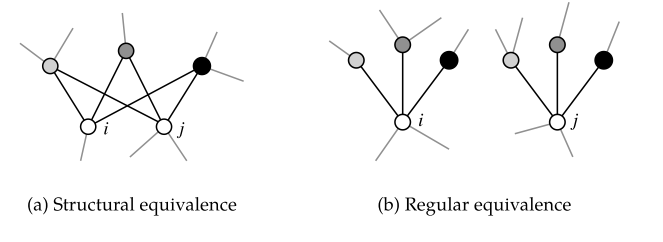
\includegraphics[width=.8\linewidth]{reg_struct_equivalence}
		\caption{Two types of similarity indices highly used in social networks, which have been applied also to food webs. As you can see, two nodes are regularly equivalent if they are connected to similar nodes (b) and structurally equivalent if they are connected to the same exact nodes (a). Two nodes that are structurally equivalent are also regularly equivalent, but not the other way around. For example, two nurses are regularly equivalent becuase they have the same connections to other personell in the hospital such as doctors, other nurses, receptionists, patients and so on. If the personell they are in contact not only is similar but it's the same exact persons, then they are also structurally equivalent.}
		\label{fig:equivalences}
	\end{figure}
	\begin{figure}[htbp]%{\textwidth}
		\centering
		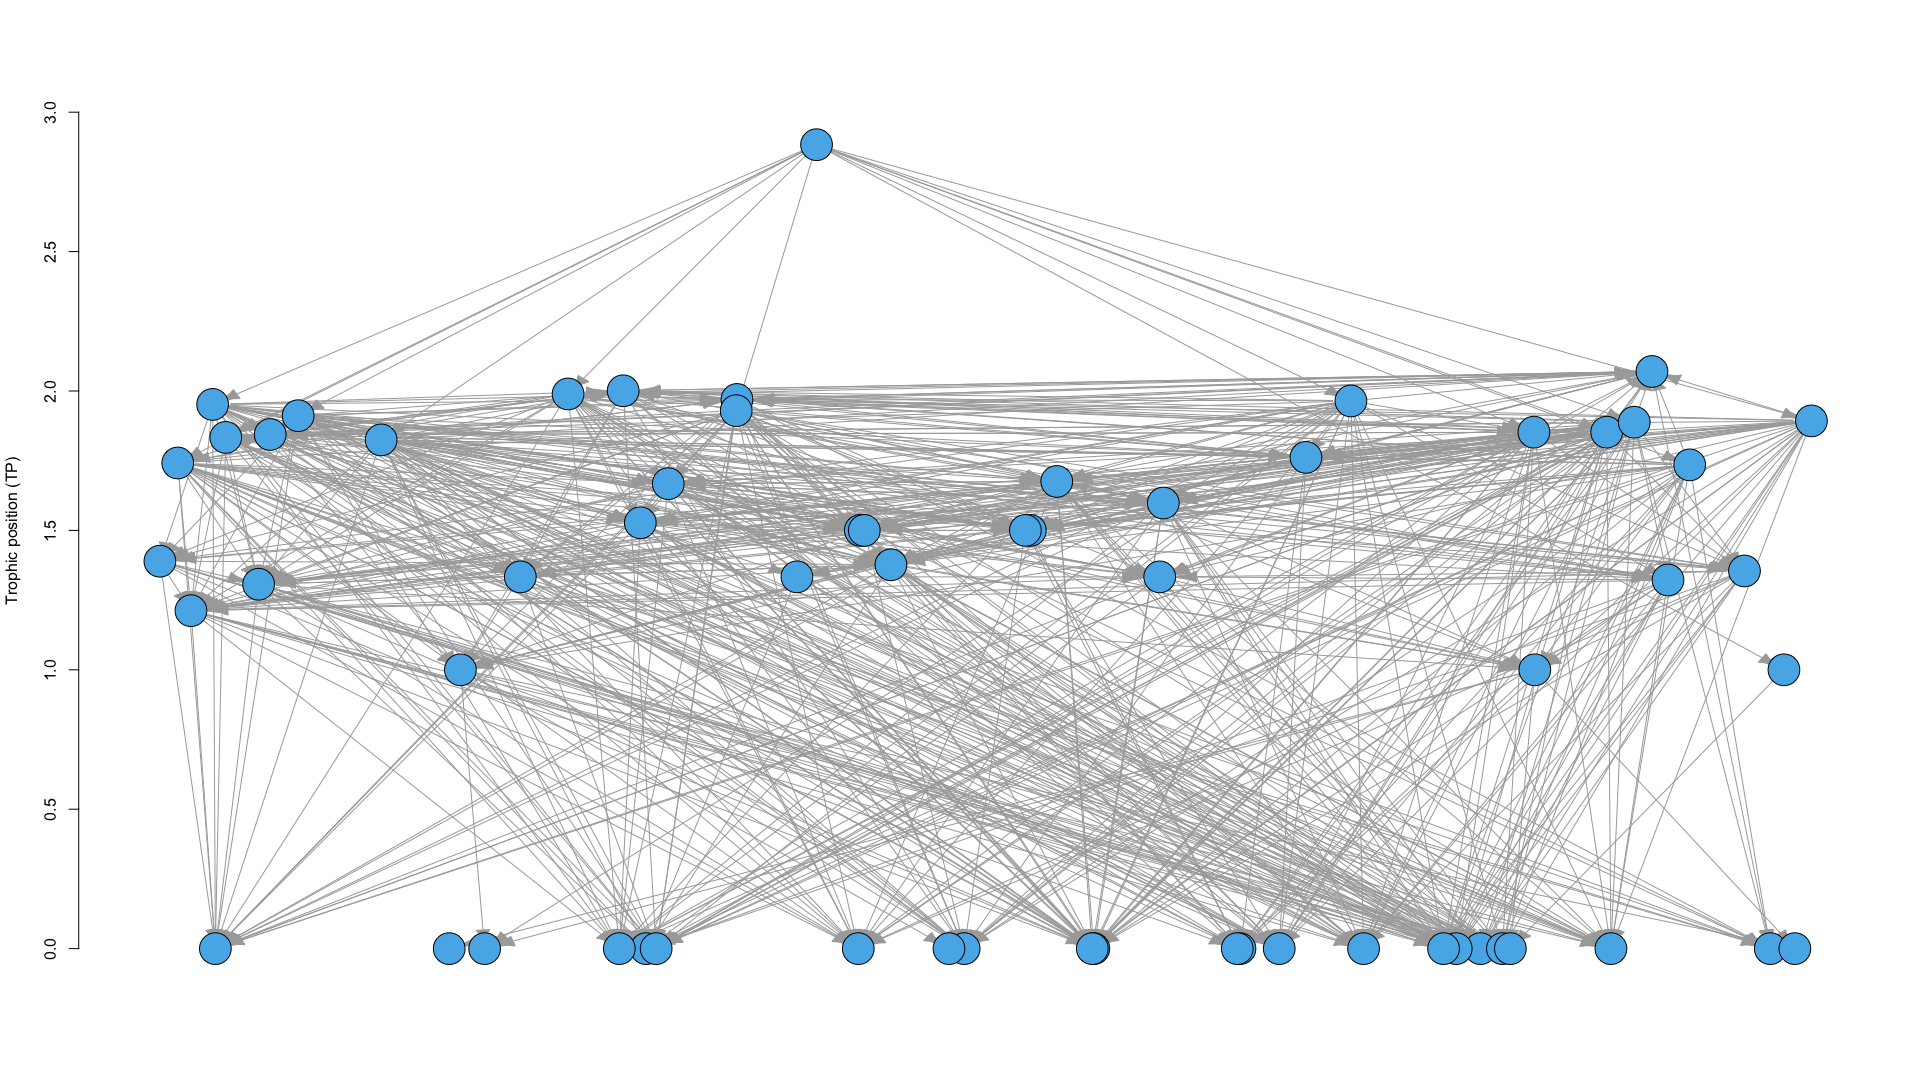
\includegraphics[width=.8\linewidth]{original_food_web.png}
		\caption{The plankton food web of the Gulf of Naples before the aggregation of its nodes (data from \citet{DAlelio2016}). The self-loops have been omitted from the figure to make it clearer.}
		\label{fig:originalweb}
	\end{figure}
\section*{Methods: clustering techniques}
	\subsection*{Hierarchical clustering of nodes according to their Jaccard similarity index}
	As a first clustering method, we clustered structurally equivalent nodes as in \citet{Yodzis1999}, using the Jaccard similarity index as a measure of structural equivalence. The clustering algorithm can be found in the appendix.
	\subsection*{Hierarchical clustering of nodes according to their REGE index}
	As a second clustering method, we clustered regularly equivalent nodes as in \citet{Luczkovich2003}, using REGE index as a measure of regular equivalence. The clustering algorithm cna be found in the appendix.
	\subsection*{Clustering of density-based modules}
		\par
		As a third clustering method, we clustered the nodes inside the modules found by maximising the density-modularity, as in \citet{Guimera2010}. This type of modularity is expressed as the number of extra links present within the modules compared to the ones expected by chance. For directed networks, it can be expressed through the following equation of \citet{Arenas2007}, which is a generalisation of the Newman-Girvan modularity \citep{Newman2004}:
			\begin{equation}
				Q=\frac{1}{L}\sum\limits_{ij}[A_{ij}-\frac{k_i^{in}k_j^{out}}{L}]\delta_{m_im_j} \label{eqn:modularitydensity}
			\end{equation}
		where $Q$ is the directed modularity of partition P, $L$ is the number of links in the network, $A_{ij}$ is the element of the adjacency matrix of a directed, binary network (links go from $j$ to $i$), $k_i^{in}k_j^{out}/L$ is the probability of having an edge between $i$ and $j$, $k^{in}_i$ is the indegree of $i$ and $k^{out}_j$ is the out-degree of $j$), $ m_i$ is the module of $i$, and $\delta$ is the Kronecker delta \citep{Kozen2007}.
		\par
		The number and composition of the modules were found by using the spectral optimisation algorithm of \citet{Leicht2008}. This algorithm is based on the principle that if we keep subdividing every module into the two modules that maximise modularity the most, we reach a point when a further subdivision would not increase the modularity anymore, giving us the most accurate modules.
	\subsection*{Clustering of prey-based and predator-based modules}
		As fourth and fifth clustering methods, we clustered the nodes of every module that was found by maximising the prey-modularity and the predator-modularity of the food web, as in \citet{Guimera2010}. In this case, the modularity of the food web is expressed as to how much different nodes connect to the same predators (for prey-modularity) or preys (for predator-modularity) than expected by chance. Mathematically, it can be expressed by the following equation \citep{Guimera2007} for prey-modularity
		\begin{equation}
			Q=\sum_{ij}{\left[\frac{c_{ij}^{out}}{\sum_{l}{k_l^{in}\left(k_l^{in}-1\right)}}-\frac{k_i^{out}k_j^{out}}{\left(\sum_{l} k_l^{in}\right)^2}\right]\delta_{m_im_j}}
		\end{equation}
		or in the following one for predator-modularity
		\begin{equation}
			Q=\sum_{ij}{\left[\frac{c_{ij}^{in}}{\sum_{l}{k_l^{out}\left(k_l^{out}-1\right)}}-\frac{k_i^{in}k_j^{in}}{\left(\sum_{l} k_l^{out}\right)^2}\right]\delta_{m_im_j}}
		\end{equation}
		where $c_{ij}^{out}$ is the number of outgoing links that i and j have in common and $c_{ij}^{in}$ is the number of incoming links that i and j have in common. For simplicity, we used the same spectral optimisation algorithm to maximise also this type of modularity. However, simulated annealing might give faster results \citep{Guimera2007}.
	\subsection*{Group model}
		\par
		As a sixth clustering method, we clustered the nodes inside the modules found by the group model of \citep{Allesina2009a}. This model finds the modules that maximise the probability of randomly retrieving the food web by generating an Erdős-Rényi random graph. For an arbitrary number of groups k, the probability of retrieving  the food web is:
		\begin{equation}
			P(N(S,L)|\vec{p}^{\,})=\prod_{i=1}^k\prod_{j=1}^k p_{ij}^{L_{ij}} (1-p_{ij})^{S_i S_j - L_{ij}}
		\end{equation}
		where $N(S,L)$ is the food web N with S number of nodes and L number of links,  $\vec{p}^{\,}$ is the vector containing the probabilities of a connection between and within clusters, $p_{ij}$
		is the probability that a node inside the group $i$ connects to another node inside the group $j$, $L_{ij}$ is the number of links connecting nodes belonging to the group i to nodes belonging to the group j, $S_i$ is the number of nodes in the cluster i,  and $S_j$ is the number of nodes in the cluster j.
		\par
		Becuase of the high number of possible module arrangments, it is not possible to explore them all.
		To find the best possible solution our computation power allows us to find, we used the algorithm of \citet{Sander2015}.
		This relies on a Metropolis-Coupled Markov Chain Monte Carlo ($MC^3$), also known as parallel tempering(Geyer, 1991), with a Gibbs sampler (Yildirim, 2012).
		$MC^3$ can be considered as a Markov chain Monte Carlo (MCMC) with multiple chains running all at once \citep{Sander2015}.
\section*{Methods: connecting modules}
	\par
	The wiring of the food web followed a similar approach to the one describe in \citep{Martinez1991}: two clusters were connected only if a certain number of links between their nodes was realised. The minimum number was one, where two clusters were connected if there was also just one connection between a member of the first cluster and a member of the second cluster.	The maximum number was 100\%, where two clusters were connected only if there was a connection between every member within a cluster and every member of the other cluster.	The numbers in between went from 1\% to 99\% with a growth rate of 1\%.	The weight of the link was then calculated in four different ways: as the minimum weight, the maximum weight, the mean weight, and the sum of the weights of the links going between the memebers of the first and the second cluster. This produced 404 food webs for each aggregation method (101 link percentages x 4 weight methods = 404 wiring options).
	\par
	For each centrality index, we compared the ranking of the nodes between the original food web and the aggregated food webs.	This was done by using Kendall's tau b ($\tau_B$),  a version of the Kendall rank correlation coefficient that makes adjustments for ties \citep{Agresti2012}.	The $\tau_B$ was calculated through the package "Mann-Kendall Tau-b with Sen's Method (enhanced)" available for MATLAB \citep{Burkey2021}. This allowed us to select the food web with the best link ratio and the best weight method for every combination of centrality index and aggregation (e.g., the status index for group model).
\section*{Methods: centrality indices}
	\subsection*{Degree centrality (DC)}
		\par
		The degree centrality (DC) is the number of links a node has \citep{Wasserman1994}
					\begin{equation}
								DC_i=\sum_{j=1}^{n}A_{ij}
					\end{equation}
		where $DC_i$ is the degree centrality of the node i, n is the number of nodes in the food web, and $A_{ij}$ is the element of the adjacency matrix, after the network has been transformed in a binary undirected one.
		It can be normalised by dividing it by the total number of possible connections that a node could have \citep{Wasserman1994}
					\begin{equation}
								nDC_i=\frac{DC_i}{n-1}\ \ \
					\end{equation}
		where n-1 is the maximum number of connections the node can have (the minus one shows that a node cannot have a connection to itself).
		\par
		Another type of degree centrality that we considered was the weighted degree centrality (wDC), often referred to as node strength. Its formula, as well as the formula of its normalised version, are the same as for the non-weighted degree centrality. This time, however, the adjacency matrix is of an undirected weighted network \citep{Fornito2016}
					\begin{equation}
								WDC_i=\sum_{j=1}^{n}A_{ij}
					\end{equation}
	\subsection*{Closeness centrality (CC)}
		\par
		The closeness centrality (CC) is the average distance a node is from all the others \citep{Wasserman1994}
					\begin{equation}
								CC_i=\frac{1}{\sum\limits_{j=1}^n d(i,j)}
					\end{equation}
		where d(i,j) is the distance between node i and j. It can be normalised as follows \citep{Wasserman1994}
					\begin{equation}
								nCC_i=\frac{n-1}{\sum\limits_{j=1}^n d(i,j)}
					\end{equation}
	\subsection*{Betweenness centrality (BC)}
		The betweenness centrality (BC) is the average number of times that a node acts as a bridge along the shortest path between two other nodes, which is mathematically expressed as follows \citep{Wasserman1994}
		\begin{equation}
			BC_i=\sum_{i\neq m\neq n}\frac{\sigma_{mn}\left(i\right)}{\sigma_{mn}}
		\end{equation}
		where $\sigma_{mn}$ is the total number of shortest paths going from s to t and $\sigma_{mn}\left(i\right)$ is the total number of these paths passing through i.
		It can be normalised with the following equation \citep{Wasserman1994}
		\begin{equation}
			nBC_i=\frac{BC_i}{\left(n-1\right)\left(n-2\right)/2}
		\end{equation}
	\subsection*{Status index (s)} The status index of a node is the sum of its distances from all the other nodes inside the network, calculated as their shortest paths following a bottom-up direction \citep{Endredi2018} \begin{equation} s_i=\sum_{j=1}^{n}d\left(i,j\right) \end{equation} It was first  introduced to social networks, followed two years later by its application to food webs by \citet{Harary1959, Harary1961}.
		By following the same method but in a top-down direction we obtain the controstatus $(s_i’)$ \begin{equation} s_i^\prime=\sum_{j=1}^{n}d\left(i,j\right) \end{equation} The difference between the status and the controstatus is called the net status ($\Delta s_i$) \begin{equation} \Delta s_i=s_i-s_i^\prime \end{equation} \subsection*{Keystone index (K)} The keystone index was firstly introduced by \citet{Jordan1999} and inspired by the status index.
		As the net status index, the keystone index of a species i (K(i)) is calculated by considering separately the bottom-up (like the status index), as well as the top-down (like the controstatus index) effects of a node \citet{Jordan2006} \begin{equation} K\left(i\right)=K_b\left(i\right)+K_t\left(i\right) \end{equation} where $K_b\left(i\right)$ is its bottom-up keystone index of species $i$ and $K_t\left(i\right)$ the top-down keystone index of species i.
		Unlike the status index, which only considers the distance between a node and all the other nodes, the keystone index takes into consideration how the size of a certain effect gets split between the different neighbours of a node.
		Every time the effect reaches a certain node connected to multiple nodes, the following nodes receive only a fraction of the total effect.
		For example, when considering the bottom-up effect, if the prey has two predators, the bottom-up effect received by each predator will be half.
		The bottom-up effect of a certain node $(K_b\left(i\right)) i$ is then calculated in the following way \begin{equation} K_b\left(i\right)=\sum_{j=1}^{n}\frac{1}{m\left(i\right)\left(j\right)}+\frac{K_b\left(j\right)}{m\left(i\right)\left(j\right)} \end{equation} where $j$ is a predator of $I$,$m(i)(j)$ is the number of preys of $j$, and $\frac{K_b\left(j\right)}{m\left(i\right)\left(j\right)}$ is the fraction of bottom-up effects of $j$ that are caused by $i$.
		The $K_b\left(j\right)$of top predators is set as 0.
		The top-down effect of a certain node $K_t\left(i\right)$ is calculated exactly as $K_b\left(i\right)$, but with the direction of the links inverted.
		\par
		The bottom-up and the top-down effects can also be split into their direct and an indirect component.
		The indirect component takes into consideration the bottom-up effects of the predator and direct component does not \begin{equation} K_{b,indirect}\left(i\right)=\sum_{j=1}^{n}\frac{1}{m\left(i\right)\left(j\right)}+\frac{K_b\left(j\right)}{m\left(i\right)\left(j\right)} \end{equation} \begin{equation} K_{b,direct}\left(i\right)=\sum_{j=1}^{n}\frac{1}{m\left(i\right)\left(j\right)}+\frac{1}{m\left(i\right)\left(j\right)} \end{equation} The direct and indirect components of the top-down effect are calculated in the same way, but with the direction of the links inverted.
		The direct and indirect keystone indices of a node are the sum of its direct/indirect bottom-up effects and its direct/indirect top-down effects \begin{equation} K_{direct}(i)=K_{b,direct}+K_{t,direct} \end{equation} \begin{equation} K_{indirect}(i)=K_{b,indirect}+K_{t,indirect} \end{equation} The keystone index not only is the sum of its top-down and bottom-up effects, but also the sum of its direct and indirect effects \begin{equation} K\left(i\right)=K_{dir}\left(i\right)+K_{indir}\left(i\right) \end{equation} \subsection*{Topological importance (TI)} The topological importance of a node represents its potential to create bottom-up effects on other species, up to a certain number of steps that we can set.
		It was first  introduced to host-parasitoid networks by \citet{Muller1999} and then to food webs by \citet{Jordan2003}.
		The algorithm of its computation is as follows \citep{Jordan2009}: \begin{enumerate} \item \emph{Compute the one-step matrix.
			      } \smallskip \newline
			      In the one-step matrix, if the energy flows from a prey to the predator, then the effect of the prey on the predator is the reciprocal of the indegree of the predator
			      \begin{equation}
				      a_{1,ij}=\frac{A_{ij}}{D_j}
			      \end{equation}
			\item \emph{Compute the n-step matrices.} \smallskip \newline
			      In the higher steps matrices, a node influences another node at a higher trophic level by summing the effects of every path that connects the two nodes.
			      The effect of every path is the multiplication of the inverse of the outdegree of every node along the path.
			      For a visual explanation see Figure \ref{fig:TI}.
			      It can be calculated as follows
			      \begin{equation}
				      A\left(n\right)=A_{\left(1\right)}^n
			      \end{equation}
			\item \emph{Calculate topological importance} \smallskip \newline The topological importance of a node i ($TI_i$) can be calculated through the following formula
			      \begin{equation}
				      TI_i=\frac{\sum\limits^N_{m=1}\sum\limits^n_{j=1}a_{m,ji}}{N}
			      \end{equation}
			      where $N$ is the total number of steps considered, $m$ is the step number,  $n$ is the total number of nodes, and $a_{m,ji}$ is the effect of species $i$ on species $j$ at $m$ number of steps.
			      \begin{figure}[htbp]%{\textwidth}
				      \centering
				      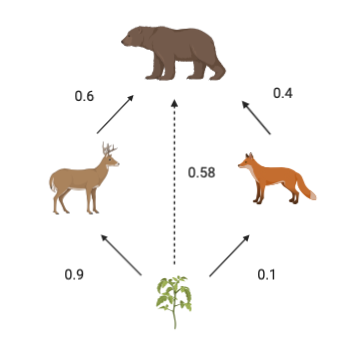
\includegraphics[width=.8\linewidth]{TI_example.png}
				      \caption{Topological importance (TI) of a species on another. The plant and the bear are not connected, so there is no direct effect from the plant to the bear. However, indirect effects reach the bear from the plant through two paths and the final effect is the sum of these effects. The first one is through the deer and the second is through the fox. The strength of these paths is the product of the direct effects composing the path. The first path has an effect on the bear that is 0.9*0.6=0.54, the second one has an effect on the bear that is 0.1*0.4=0.04. Summing the effects through these two 2-step paths connecting the plant with the bear, we get the 2-step effect of the plant on the bear: 0.54+0.04=0.58. Figure created with BioRender.com.}    \label{fig:TI}
			      \end{figure}
		\end{enumerate}
		\par
		Topological importance can be also used for weighted networks - giving us weighted topological importance ($WI$) – if instead of using the degree ($D$) we use the weighted degree ($WD$) \citep{Scotti2007} \begin{equation} a_{1,ji}=\frac{A_{ij}}{weighted\:indegree_j} \end{equation} where $A_{ij}$ is the element of the adjacency matrix of the weighted directed network.
	\subsection*{Trophic field overlap (TO)}
		The trophic field overlap (TO) represents how redundant the strong interactions of a node are.
		It was first  introduced by \citet{Jordan2009a}.
		It is the number of times that it and another node interact strongly with the same predator.
		The algorithm for its computation is the following one \citep{Jordan2018}:
		\begin{enumerate}
			\item Compute the one-step matrix as in toplogical importance \item Compute the n-step matrix as in topological importance \item Compute the average effect matrix.
			      The average effect matrix ($E(n)$) represents the effect of each node on the other nodes average by the number of steps
			      \begin{equation}
				      E_n=\frac{1}{n}\sum_{i=1}^{n}A_{\left(i\right)}
			      \end{equation}
			\item Compute the interactor matrix.
			      Compute the so-called interactor matrix ($M_T$), whose values tell us whether the interaction between two nodes is weak (W) or strong (S).
			      To do this, we need to define a threshold over which a certain interaction is strong.
			\item Compute the topological overlap matrix.
			      Compute a matrix with how many times two species interact strongly with the same predator, called the topological overlap matrix.
			\item Compute the trophic field overlap (TO)
			      The trophic field overlap (TO) of a node is calculated by summing the elements of the rows of the topological overlap matrix.
		\end{enumerate}
		Trophic field overlap can be also used for weighted networks – giving us weighted trophic field overlap (WO) – if instead of using the degree (D) we use the weighted degree, (e.g.,  \citet{Xiao2019})
		\begin{equation}
			a_{1,ij}=\frac{A_{ij}}{D_j}
		\end{equation}
		Finally, to avoid the bias of choosing a wrong threshold, we chose multiple thresholds and summed the TO of a species i for each of these thresholds.
		This gave us the species uniqueness (STO), an index that was firstly introduced by \citet{Lai2015}.
	\subsection*{Trophic position (TP)}
		The trophic position of a node is the mean length connecting it to the producers of the ecological community (its energy source). It was firstly introduced by \citet{Levine1980}, as a generalization of the earlier use of integer trophic levels to include cycles and fractional positions. It can be calculated through the following formula
		\begin{equation}
			TP_i=\sum\limits_{k=0}^\infty k \cdot p_i(k).
		\end{equation}
		where $k$ is a certain path length and $p_i(k)$ is the probability that species $i$ will reach the energy produced by the autotrophs via a path of length $k$. $TP$ equals 0 for producers, it equals 1 for herbivores and larger values for omnivores and carnivores.
\section*{Results \& discussion}
	We are still in the process of writing the results and the discussion of this paper. I thought, however, that it would have been informative to upload my most recent work to show you what I am doing at the moment.
\section*{Acknowledgements}
	We would like to thank Wei-Chung Liu for providing the code for computing some centrality indices and Stefano Allesina \& Elizabeth Sander for providing the code for the  computation of the group model.
	\bibliographystyle{apalike}
	\bibliography{/Applications/Mendeley/library.bib}
\begin{appendices}
	\section{Hierarchical clustering with Jaccard similarity index}
	\label{appendix:a}
		\begin{enumerate}
			\item \emph{Compute similarity.} \smallskip \newline
						Compute the Jaccard similarity between the nodes by using the following equation \citep{Yodzis1999}:
						\begin{equation}
				      J_{ij}=\frac{a}{a+b+c} \label{eqn:jaccard}
			      \end{equation}
			      where $J_{ij}$ is the Jaccard similarity between node $i$ and $j$, $a$ is the number of preys and predators that $i$ and $j$ have in common, $b$ is the number of preys and predators exclusively of i, and $c$ is the number of preys and predators exclusively of $j$.
			\item \emph{Build the dendrogram.} \smallskip \newline
			      Find the two most similar elements and cluster them together (elements are intended as nodes or clusters. Of course, the first time we run this step all the elements are nodes). Repeat until you are left with only one item, which is the final dendrogram. During this process, the similarity between two clusters can be calculated in different ways, called linkage criteria. The ones that we used were
			      \begin{itemize}
				      \item 	The similarity between the least similar nodes, one in each cluster, known as \textbf{single-linkage} \citep{Frigui2008}.
				      \item 	The similarity between the most similar nodes, one in each cluster, known as \textbf{complete linkage} \citep{Frigui2008}.
				      \item 	The mean similarity between the nodes inside the first item and the second item, known as the \textbf{weighted average distance(WPGMA)} \citep{Sokal1958}:
				            \begin{equation}
					            d_{(i \bigcup j),k}=\frac{d_{i,k}+d_{j,k}}{2} \label{eqn:WPGMA}
				            \end{equation}
	            where $d_{\left(i\cup j\right),k}$ is the distance between the cluster $i \bigcup j$ (cluster including $i$ and $j$) and $k$, $d_{i,k}$ is the distance between $i$ and $k$, and  $d_{j,k}$ is the distance between $j$ and $k$.
				      \item	The mean similarity between the nodes inside the first item and the second item, but taking into consideration the average distance between the items inside the fist cluster;
				            this is known as the\textbf{unweighted average distance (UPGMA)} \citep{Sokal1958}:
				            \begin{equation}
					            d_{(i \bigcup j),k}=\frac{|i|d_{i,k}+|j|d_{j,k}}{|i|+|j|} \label{eqn:UPGMA}
				            \end{equation}
										where $|i|$ and $|j|$ are the mean distances between the elements inside $i$ and $j$, respectively.
			      \end{itemize}
			\item \emph{Select the dendrogram.} \smallskip \newline
						After having produced a dendrogram for every linkage criteria, select the dendrogram with the highest cophenetic correlation \citep{Sokal1962}.
			      This allows selecting the linkage criterion that produces the dendrogram that preserves the most faithfully the pairwise similarity between different elements.
			\item \emph{Cut the dendrogram.} \smallskip \newline
			      Cut the dendrogram according to the maximum inconsistency of the branches, set at 0.01.
		\end{enumerate}
		\section{Hierarchical clustering with REGE index}
		\label{appendix:b}
		\begin{enumerate}
				\item \emph{Compute similarity.} \smallskip \newline
							Compute the similarity between nodes by using REGE, calculated by the homonym algorithm. This was originally developed in the unpublished work by \citet{White1980,White1982,White1984} and firstly described in the literature by \citet{Borgatti1993}. It is available to be used in the software UCINET VI \citet{Borgatti2002}. The REGE algorithm is as follows \citep{Jordan2018}:
				      \begin{enumerate}
					      \item Set the maximum number of iterations. We set 3 iterations. Each iteration produces a matrix $R_{\left(t\right)}$ where $t$ is the number of the iteration and every element $r_{\left(t\right)ij}$ is the regular equivalence between i and j at iteration t. The regular equivalence between nodes at iteration t=0 is always 1.
					      \item Starting from t=1, update the elements of the matrix following these sub-steps:
					            \begin{enumerate}
						            \item For every predator k of species i, find the most similar predator m of species j according to  $R_{\left(t\right)}$.
						                  Now, set $X_{i,k,j}=R_{\left(t\right)km}.
						                  $
						            \item For every predator m of species j, find the most similar predator k of species o according to $R_{\left(t\right)}$.
						                  Now, set $X_{j,m,i}=R_{\left(t\right)mk}$.
						            \item For every prey h of species i, find the most similar prey n of species j according to $R_{\left(t\right)}$.
						                  Now, set $Y_{i,h,j}=R_{\left(t\right)hn}$.
						            \item For every prey n of species j, find the most similar prey h of species i according to $R_{\left(t\right)}$.
						                  Now, set $Y_{j,n,i}=R_{\left(t\right)nh}$.
						            \item Update the matrix R through the following equation
						                  %\begin{equation}
						                  % R_{\left(t\right)ij}=\frac{\sum_{k=1} X_{i,k,j}+\sum_{m=1} X_{j,m,i}+\sum_{h=1} Y_{i,h,j}+\sum_{n=1} Y_{j,n,i}}
						                  %{MAX\left(\sum_{k=1} X_{i,k,j}+\sum_{m=1} X_{j,m,i}+\sum_{h=1} Y_{i,h,j}+\sum_{n=1} Y_{j,n,i}\right)}
						                  %\end{equation}
						            \item Increase t=t+1 and repeat step b until you reach the maximum number of iterations. The matrix of the maximum number of iterations contains the regular equivalence between nodes.
					            \end{enumerate}
					      \item Increase t=t+1 and repeat step b until you reach the maximum number of iterations. The matrix of the maximum number of iterations contains the regular equivalence between nodes.
				      \end{enumerate}
				\item \emph{Build the dendrogram.} \smallskip \newline
							The same as in the hierarchical clustering of nodes according to their Jaccard similarity index. During our analysis, we used the function linkage of MATLAB, which does not include the possibility of using a similarity matrix, so we converted the similarity matrices into dissimilarity ones. This was done by following what was written in \citet{VonLuxburg2004}. Namely, if the similarity function is normalised - takes values between 0 and 1 - and always positive, then $d=1-s$ where d is the dissimilarity measure and s is the similarity measure).
				\item \emph{Select the dendrogram.} \smallskip \newline
							The same as in the hierarchical clustering of nodes according to their Jaccard similarity index.
				\item \emph{Cut the dendrogram.} \smallskip \newline
				      The same as in the hierarchical clustering of nodes according to their Jaccard similarity index.
		\end{enumerate}
\end{appendices}
\end{document}
